% =====================================================================
% Figura 8 — Localização da área de coleta.
%
% Substitui mapa_bambui.png (764x547 px, cerca de 129 dpi na largura de
% texto). A imagem de satélite foi recortada e teve os rótulos de baixa
% resolução removidos; a rotulagem é refeita aqui em vetor, de modo que
% os nomes dos sítios permanecem nítidos em qualquer ampliação.
%
% REQUER no preâmbulo (já presentes em artigo.tex):
%   \usepackage{tikz}
%   \usetikzlibrary{positioning, arrows.meta}
% =====================================================================

\begin{figure}[H]
    \centering
    \caption{Localização geográfica da região de coleta das imagens em
             Bambuí, Minas Gerais: (a) posição das duas propriedades em
             relação à sede do município; (b) entrada da Fazenda Trevo;
             (c) talhão de café em produção}
    \label{fig:mapa_bambui}

    \begin{tikzpicture}[
        placa/.style={
            fill=white, fill opacity=0.88, text opacity=1,
            rounded corners=1.5pt, inner xsep=3pt, inner ysep=2.2pt,
            font=\scriptsize, text=black, anchor=center
        },
        marca/.style={draw=white, line width=0.6pt, fill=black!80},
        letra/.style={
            fill=black, fill opacity=0.65, text opacity=1, text=white,
            font=\scriptsize\bfseries, inner sep=2pt,
            rounded corners=1pt, anchor=north west
        }
    ]

    % ------------------------------------------------- (a) recorte aéreo
    \node[anchor=south west, inner sep=0] (mapa) at (0,0)
        {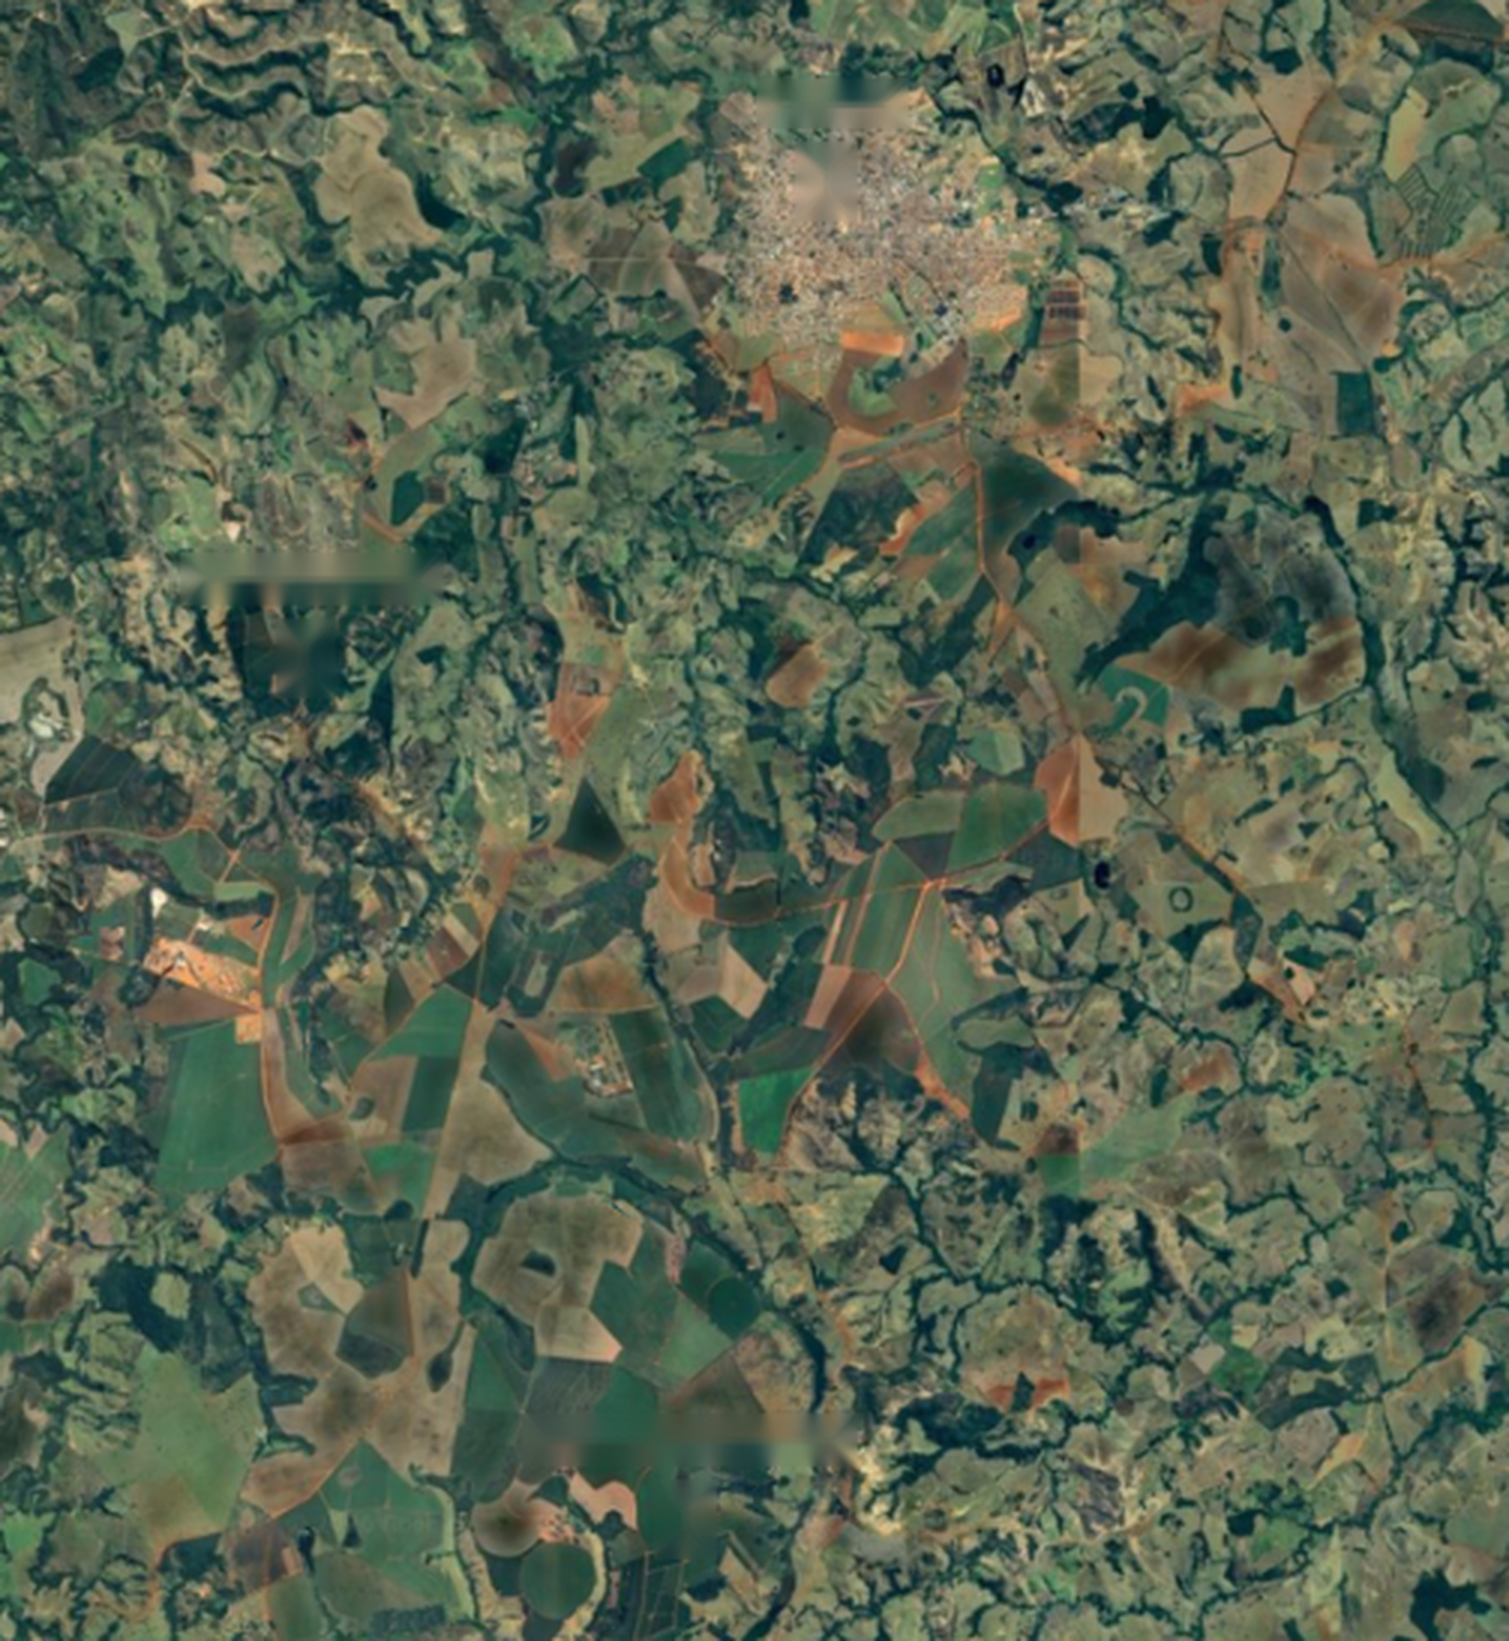
\includegraphics[width=8.40cm]{figuras/mapa/mapa_limpo.png}};

    % alfinetes: disco sobre o ponto, com haste apontando a posição exata
    \foreach \px/\py in {4.601/7.899, 1.703/5.244, 3.816/0.451}{%
        \fill[marca] (\px,\py) -- ++(-0.105,0.27) -- ++(0.21,0) -- cycle;
        \filldraw[marca] (\px,{\py+0.29}) circle (0.16);
        \fill[white] (\px,{\py+0.29}) circle (0.055);
    }

    % rótulos dos sítios
    \node[placa] at (4.634,8.559) {Bambuí};
    \node[placa] at (1.737,5.912) {Fazenda Trevo};
    \node[placa] at (3.841,1.119) {Fazenda do Lazinho};

    \node[letra] at (0.10,9.03) {a};

    % ------------------------------------------------ (b) e (c) fotos
    \node[anchor=north west, inner sep=0] (fb) at (8.62,9.135)
        {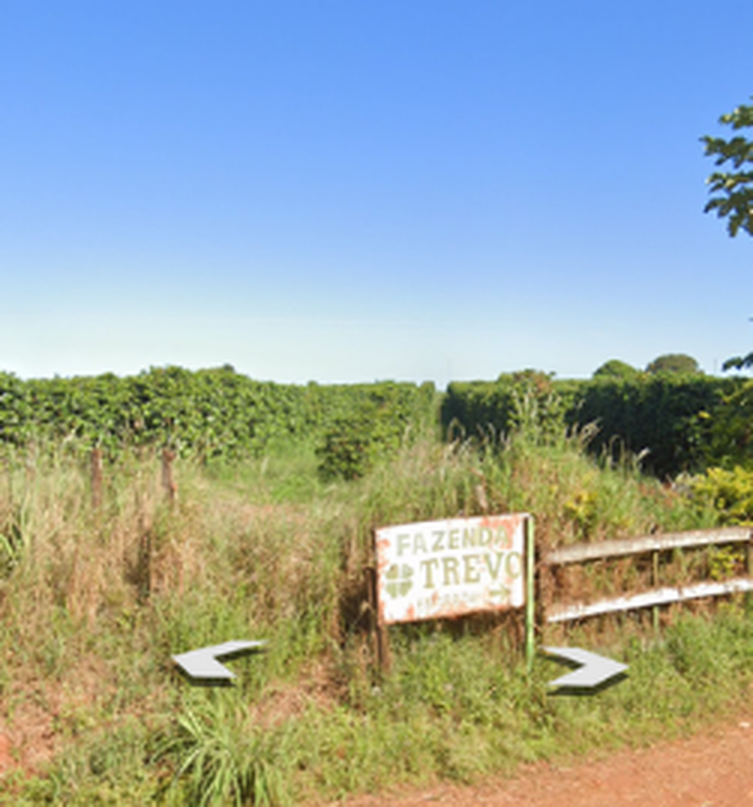
\includegraphics[width=4.18cm]{figuras/mapa/foto_placa.png}};
    \node[anchor=north west, inner sep=0] (fc) at (8.62,4.49)
        {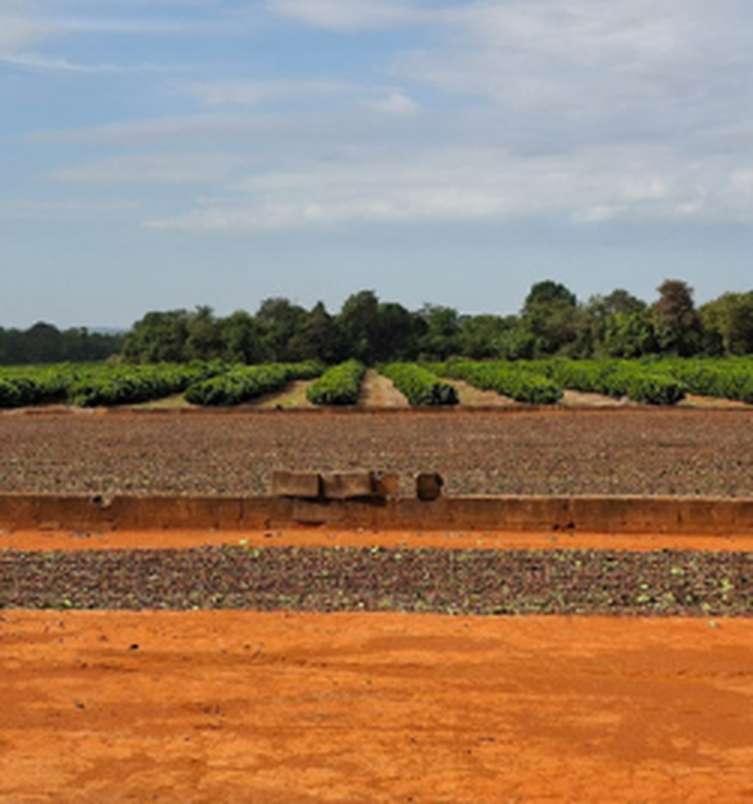
\includegraphics[width=4.18cm]{figuras/mapa/foto_lavoura.png}};

    \node[letra] at ([shift={(0.07,-0.07)}]fb.north west) {b};
    \node[letra] at ([shift={(0.07,-0.07)}]fc.north west) {c};

    \end{tikzpicture}

    \legend{Elaborada pela autora (2026), sobre imagem de satélite do
            Google Earth.}
\end{figure}
